\documentclass{article}

\IfFileExists{neurips_2027.sty}{
  \usepackage[preprint]{neurips_2027}
}{
  \usepackage[margin=1in]{geometry}
}
\usepackage[utf8]{inputenc}
\usepackage[T1]{fontenc}
\usepackage{amsmath,amssymb}
\usepackage{booktabs}
\usepackage{graphicx}
\usepackage{placeins}
\usepackage{float}
\usepackage{hyperref}

\newcommand{\inputrepoartifact}[1]{%
  \IfFileExists{../../#1}{%
    \input{../../#1}%
  }{%
    \input{#1}%
  }%
}
\newcommand{\inputoutlierartifact}[1]{\inputrepoartifact{outputs/outlier_pair/#1}}
\newif\ifrancanonymous
\ifdefined\rancanonymoussubmission
  \rancanonymoustrue
\else
  \rancanonymousfalse
\fi

\title{RANC-ContractNet: Auditable Normalization as Invariance Compilation}

\ifrancanonymous
\author{
  Anonymous Author \\
  Anonymous Institution \\
  \texttt{anonymous@example.org}
}
\else
\author{
  Harshad Hemant Patil \\
  Lead Data Scientist, Springer Nature \\
  \texttt{hhpatil001@gmail.com}
}
\fi

\begin{document}

\maketitle

\begin{abstract}
Normalization is often treated as a preprocessing hyperparameter, but every
normalizer encodes a legality claim: which variation may be removed, and which
signal must survive. Validation-score scaler search can hide illegal choices: a
rank map can erase metric signal, robust scaling can damp rare positives,
centering can densify sparse inputs, and fitting outside the active training
fold can leak future information. RANC-ContractNet treats normalization as
invariance compilation rather than AutoML scaler search. Given a training fold,
an explicit contract, and implemented checkers, it builds regime cards, records
signal-risk ledger rows, selects the least complex admissible policy, and gates
acceptance with falsification tests. The fitted sklearn transformer returns
transformed data together with a replayable audit report containing fitted
statistics, rejected candidates, downgrades, drift monitors, and test outcomes.
The guarantee is relative to the declared contract: accepted policies pass
checked hard clauses, while failures become recorded downgrades or no-ops. In
paired outlier worlds where identical extremes are either noise or rare signal,
correct contracts improve the targeted failure metric over wrong-contract
controls. The claim is auditable legality under declared invariances and
implemented checkers, not universal predictive dominance.
\end{abstract}

\section{Introduction}

Most machine-learning pipelines name a normalizer but not the contract that
licenses it. Standardization declares mean and scale expendable. Robust scaling
declares extremes suspicious. Rank transforms preserve order while discarding
metric gaps. Centering sparse features may change both storage and semantics.
These are semantic decisions, not cosmetic preprocessing. A validation metric
can reward a transform that is useful for one split and still illegal for the
task because it removed declared signal, violated representation constraints, or
used information that should not have been visible.

The missing object is a contract. Before a normalizer is fit, a pipeline should
be able to state which observations may supply statistics, which invariances are
allowed, which feature geometry must remain valid, whether an inverse is
required, and whether rare extremes are corruptions or signal. A validation
selector answers a different question: which scaler helped a downstream model on
a held-out split? That may be useful, but it does not certify that the selected
transform preserved zeros, avoided leakage, respected temporal order, or kept
declared rare signal intact.

This paper treats normalization as a compilation problem. The input is a
training fold plus a contract over invariance, signal risk, split discipline,
representation, and auditability. The output is a fitted policy and a structured
audit trail. A policy can be predictively helpful and still illegal if it
violates a hard clause; conversely, a conservative no-op can be the correct
compiled result when no candidate transform is justified by the declared
semantics.

RANC-ContractNet implements this view for tabular pipelines. It profiles only
the active training fold into regime cards, ingests or derives invariance
contracts, records candidate signal-destruction risks in a ledger, enumerates
deterministic policy families, rejects hard-clause violations, and selects the
lowest-complexity legal policy with audit-cost tie breaking. It then runs
targeted falsification tests for leakage, zero and sign preservation,
monotonicity, inverse error, outlier semantics, drift stress, covariance
distortion, sparse densification, and bounded saturation. The fitted object is a
drop-in sklearn transformer whose serialized audit report is part of the result.

The paper makes five contributions:
\begin{enumerate}
\setlength{\itemsep}{0pt}
\setlength{\parsep}{0pt}
  \item a typed contract vocabulary for regime cards, invariance clauses,
  signal-risk ledgers, policies, drift monitors, falsification results, and
  audit reports;
  \item a train-fold-only sklearn transformer with deterministic serialization
  and legal inverse behavior;
  \item a deterministic compiler over common normalization families that uses
  hard clauses rather than validation outcomes to choose a policy;
  \item falsification tests that turn failures into recorded rejections,
  downgrades, or no-ops; and
  \item a reproducible artifact path covering synthetic semantic controls,
  sparse and temporal safety checks, ablations, OpenML/UCI public runs, PDF
  rendering, and clean extracted-bundle validation.
\end{enumerate}
The claim is deliberately narrow. RANC-ContractNet is not AutoML under another
name, and it does not prove that user-supplied semantics are correct. Wrong
contracts can preserve the wrong structure; the artifact exposes this through
wrong-contract controls, signal-risk ledger rows, and degraded targeted metrics.

\section{Related Work}

\paragraph{Preprocessing libraries and statistical transforms.}
RANC-ContractNet builds on the same practical transform vocabulary exposed by
mainstream machine-learning libraries: standardization, min/max scaling,
max-absolute scaling, robust affine transforms, quantile maps, and power
transforms \cite{pedregosa2011scikit,yeo2000new}. These libraries explain how to
fit a chosen transform; they do not state whether centering violates sparse-zero
semantics, whether rank mapping erases distance-as-signal evidence, whether an
inverse is legally required, or whether fitted statistics came from an allowed
split. RANC keeps the same primitive vocabulary but changes the interface: a
scaler is selected only after it satisfies declared invariance, sparsity,
inverse, monotonicity, and audit clauses. The contribution is a legal and
auditable compiler for existing primitives.

\paragraph{AutoML and validation-selected pipelines.}
AutoML systems and pipeline optimizers search over model families,
preprocessors, and hyperparameters to improve validation performance
\cite{feurer2015automl,olson2016tpot}. Their central question is which pipeline
scores best under a search budget. RANC addresses a prior legality question:
which normalization policies are permissible before validation performance is
consulted. It compiles the least complex legal policy under a contract and audit
cost, then records rejected candidates, downgrades, no-ops, and falsification
results. A validation-selected scaler is a useful comparator and can win raw
score, but it optimizes a different target from contract compilation.

\paragraph{Leakage, documentation, and audit artifacts.}
Data leakage work motivates treating preprocessing statistics as part of the
learning procedure rather than as dataset-level constants
\cite{kaufman2012leakage}. Pipeline APIs reduce accidental full-dataset fitting,
but usually leave no normalization-specific artifact explaining which split was
visible, which clauses were required, or which candidate failed. Dataset and
model documentation efforts make assumptions, uses, and evaluation contexts
inspectable \cite{gebru2021datasheets,mitchell2019modelcards}. RANC extends this
stance to the normalization decision itself: every selected transform is paired
with the licensing contract, train-only evidence, and falsification checks.

\paragraph{Neural normalization and bounded alternatives.}
Neural normalizers act inside learned models, including BatchNorm, LayerNorm,
\mbox{GroupNorm}, and \mbox{RMSNorm}; bounded alternatives such as Dynamic Tanh
revisit whether explicit normalization layers are always required
\cite{ioffe2015batch,ba2016layer,wu2018group,zhang2019rmsnorm,zhu2025dyt}.
Those methods target optimization and representation stability. RANC's neural
path is intentionally scoped as an exploratory adapter that exposes axis choice,
centering choice, saturation, and train versus inference audit behavior under
the same contract language. The central contribution remains the preprocessing
compiler for tabular pipelines.

\section{Method}

\subsection{Problem setting}

Let $X_{\mathrm{train}}$ be the active training fold visible to a preprocessing
estimator. RANC compiles a fitted policy $P$ for later validation, test, or
deployment data using statistics from $X_{\mathrm{train}}$ and admissible
metadata only. Metadata may include feature groups, temporal context, sparse
flags, and user contracts, but not validation/test outcomes for scaler choice.
Validation search asks which preprocessing option helped a downstream model;
contract compilation asks which options are legal under declared invariance,
signal, representation, and audit requirements. If a contract is underspecified,
contradictory, or unsupported by checkers, a recorded downgrade or no-op is a
valid compiled outcome rather than a failed search.

\subsection{Formal contract semantics}

\paragraph{Definition 1 (Regime card).}
For a feature group $g$, a regime card $C_g$ is a training-only summary. It
records sample count, missingness, sparsity, sign pattern, range and boundedness,
tail evidence, drift context, local covariance context, and audit notes. Every
field is computed from $X_{\mathrm{train}}$ and allowed metadata only.

\paragraph{Definition 2 (Invariance contract).}
An invariance contract is a tuple $K_g=(H_g,A_g,I_g,R_g,S_g)$, where $H_g$ is a
set of hard predicates, $A_g$ states which observations and metadata are
admissible during fitting, $I_g$ states whether an inverse must be available,
$R_g$ records declared signal risks such as rare extremes or distance ratios,
and $S_g$ records split discipline. Typical hard predicates include zero/sign
preservation, monotonicity, sparse no-densification, bounded output, train-only
fitting, and inverse error tolerance.

\paragraph{Definition 3 (Legal normalization policy).}
A fitted policy $f_{\theta,g}$ is legal for $(C_g,K_g)$ when: (i) $\theta$
depends only on observations admitted by $A_g$ and $S_g$; (ii) every checked
$h\in H_g$ holds on the fitted policy over its declared domain or audit support;
(iii) representation constraints such as implicit sparse zeros are preserved
unless waived; (iv) required inverse error is at most
$\epsilon_{\mathrm{inv}}$ on the audit sample; and (v) selected parameters,
rejections, and downgrades are serializable. Legal does not mean predictively
optimal or semantically correct; a high-scoring policy is still illegal if it
violates a hard clause.

\paragraph{Definition 4 (Signal-risk ledger).}
The ledger $L_g$ is a set of rows
$(f,\rho,h,e,\delta)$ describing candidate transform $f$, risk type $\rho$,
affected contract clause $h$, observed evidence $e$, and decision $\delta$.
Ledger rows make destructive-but-common choices reviewable: for example, rank
maps can erase metric distances, robust scalers can suppress rare-event signal,
and centering sparse features can destroy storage semantics.

\paragraph{Definition 5 (Falsification acceptance rule).}
Let $\mathcal{T}(f_{\theta,g},C_g,K_g,L_g)$ be the required falsification tests
for leakage, zero/sign preservation, monotonicity, inverse error, outlier
semantics, drift stress, covariance distortion, sparsity, and bounded
saturation. Exact checkers certify stated domains; numeric falsification tests
certify only their deterministic audit support. RANC accepts a policy only when
it is legal and every required test passes:
\[
\mathsf{Accept}(f_{\theta,g}) =
\mathsf{Legal}(f_{\theta,g}; C_g,K_g)
\wedge
\bigwedge_{\tau \in \mathcal{T}}\mathsf{Pass}(\tau).
\]
Any required failure triggers deterministic fallback to the next simplest
candidate, downgrade to a safer policy, or an explicit no-op with recorded
reasons.

\begin{table}[t]
\centering
\scriptsize
\setlength{\tabcolsep}{5pt}
\renewcommand{\arraystretch}{0.82}
\caption{Contract clauses map directly to compiler behavior and falsification evidence.}
\label{tab:contract-evidence}
\resizebox{\linewidth}{!}{%
\begin{tabular}{ll}
\toprule
Clause & Compiler behavior and audit/falsification evidence \\
\midrule
Train-only fitting & fit active fold; record fit count, split metadata, leakage sentinels \\
Monotonicity & reject nonmonotone maps; record SMT/numeric checker and rejected candidates \\
Zero preservation & prefer identity/max-abs/no-centering; record zero test and sparse nnz delta \\
Sign preservation & reject sign crossing unless waived; record sign test and hard-clause status \\
Sparse no-densification & downgrade centering; record sparse flag, nnz before/after, densification failures \\
Inverse validity & require inverse error below tolerance; record error and inverse legality \\
Outlier-as-noise & allow monotone compression or robust damping; record ledger, policy, corruption AUROC \\
Outlier-as-signal & preserve metric tail evidence; record ledger, policy, rare-recall check \\
Temporal drift & fit prefix only; record fit count, monitor count, and max drift \\
Bounded saturation & reject or log high saturation; record saturation rate and downgrade/no-op reason \\
\bottomrule
\end{tabular}
}
\end{table}

\paragraph{Proposition 1 (relative contract soundness).}
Assume a finite candidate set, admissible-only fitted parameters, and
deterministic checkers with recorded domains or audit support. If
Algorithm~\ref{fig:ranc-algorithm} accepts $f_{\theta,g}$, then the policy used
no forbidden fitting observations, passed every required checker on stated
support, and produced an audit that replays the selected policy, rejections, and
downgrades. If no admissible candidate passes, RANC returns a recorded downgrade
or no-op rather than an unchecked policy. Proof sketch: hard-clause failures are
rejected before tie breaking, the objective ranges only over survivors, and
final falsification gates acceptance. The proposition is relative to the
declared contract and checkers; it does not prove semantic truth, downstream
optimality, or behavior outside the checked domain.

\subsection{Contract-to-policy compilation}

Given $C_j$, $K_j$, and $L_j$, RANC ranks only candidates that satisfy the hard
contract predicates. Among those legal candidates it solves
\[
P_j = \arg\min_{f \in \mathcal{F}_j}
\mathrm{complexity}(f) + \lambda_{\mathrm{audit}}\mathrm{audit\_cost}(f)
\]
subject to hard contract clauses, train-split-only fitted statistics, and
passing falsification tests. The candidate family includes identity, z-score,
robust affine, min/max, max-absolute, vector normalization, log/log1p,
power-style monotone compression, empirical rank maps, piecewise affine maps,
and optional whitening-style group policies.

The objective is a legal-policy tie breaker, not a validation-score search. If
two policies satisfy the contract, the compiler prefers the simpler and more
auditable one. Candidate statistics are estimated once from the active training
fold and then replayed unchanged at validation, test, and deployment time. When
symbolic checks are available, piecewise affine monotonicity and related hard
constraints are checked with SMT; otherwise the audit records deterministic
numeric verification and the resulting evidence limits.

\begin{figure}[t]
\centering
\fbox{\begin{minipage}{0.94\linewidth}
\small
\textbf{Algorithm 1: RANC-ContractNet fit}

\smallskip
\begin{enumerate}
\setlength{\itemsep}{0pt}
\setlength{\parsep}{0pt}
  \item Split before fitting; expose only the active training fold to the compiler.
  \item Build regime cards with missingness, sparsity, sign, range, tail, drift, and covariance summaries.
  \item Ingest user contracts or derive conservative defaults from the regime cards.
  \item Populate the signal risk ledger for each candidate transform that may erase declared signal.
  \item Enumerate deterministic candidates from $\mathcal{F}_j$ and reject hard-clause violations.
  \item Use SMT checks for piecewise affine monotonicity when available; otherwise record numeric verification.
  \item Select the minimum complexity plus audit-cost policy with deterministic tie breaking.
  \item Run falsification tests for leakage, zero/sign preservation, monotonicity, inverse error, outliers, drift, covariance, sparsity, and bounded saturation.
  \item Serialize the selected policies, rejected candidates, fitted statistics, seeds, ledgers, monitors, and falsification outcomes.
\end{enumerate}
\end{minipage}}
\caption{The compiler uses contracts rather than validation-set score search to choose a normalization policy. All fitted statistics are computed from the training fold only.}
\label{fig:ranc-algorithm}
\end{figure}

\subsection{Audit semantics}

The fitted transformer exposes transformed data and a reviewer-facing audit
object. The audit records regime cards, contracts, selected policies, rejected
candidates, ledger rows, train-only evidence, downgrades, drift monitors, and
falsification outcomes. A validation selector can report which scaler won a
metric; RANC reports why the selected transform was legal under the declared
invariances, or why it was downgraded to a safer policy.

\section{Experiments}

The experiments are organized as falsification tests for the contract-compilation
claim: whether declared semantics change legal normalization decisions and make
them auditable. The evidence chain is ordered by claim strength. The paired
outlier benchmark tests contract causality directly; Sparse and temporal checks
test representation and split-safety failures; ablations test ledger, downgrade,
and audit observability; OpenML/UCI runs test the public artifact path and
predictive scope boundary; neural pilots are exploratory.

\begin{table}[H]
\centering
\scriptsize
\setlength{\tabcolsep}{4pt}
\renewcommand{\arraystretch}{0.86}
\caption{Evidence map for the contract-compilation claim. Each row names the
claim, the failure it should expose, and the artifact that must make the result
auditable; no row is a universal scaler leaderboard.}
\label{tab:claims-tested}
\resizebox{\linewidth}{!}{%
\begin{tabular}{llll}
\toprule
Experiment & Claim tested & Failure mode exposed & Primary evidence \\
\midrule
Paired outlier worlds & contracts change legal policy & wrong semantics preserve/remove signal & correct vs wrong contract deltas \\
Sparse safety & representation clauses are enforced & centering densifies implicit zeros & sparse output, nnz delta, failures \\
Temporal drift & fitting is train-prefix only & future statistics leak into preprocessing & fit count and drift monitors \\
Ablations & audit components are observable & ledgers/downgrades disappear when removed & ledger rows, rejected candidates \\
OpenML/UCI path & public runs are reproducible and scoped & raw-score selector optimizes another target & paired deltas, exclusion log \\
Artifact checks & claims can be regenerated from package & local state or identity leaks into bundle & render, dryrun, SHA256, anonymization scan \\
\bottomrule
\end{tabular}
}
\end{table}

\begin{figure}[H]
\centering
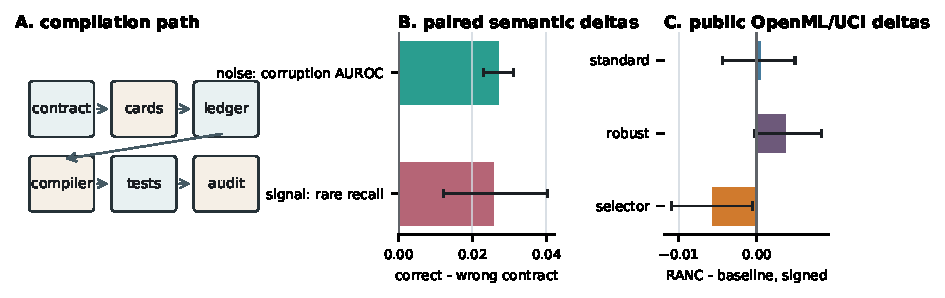
\includegraphics[width=\linewidth]{figures/ranc_visual_summary.pdf}
% Source figure data: contract_delta_table.tex and openml_win_loss_table.tex.
\caption{Visual summary of the method and two main quantitative summaries.
Panel A shows the contract-to-audit compilation path. Panel B plots the paired
semantic deltas. Panel C gives signed public-data deltas (Public-data execution
evidence on OpenML/UCI); positive values favor RANC after metric-direction
alignment, and full generated tables remain in the artifact.}
\label{fig:ranc-visual-summary}
\end{figure}

\subsection{Experimental protocol and reporting discipline}

All paper-facing experiments are config-driven. The paired outlier benchmark uses
seeds $0$--$29$, $n=800$, a 35\% stratified test split, 5,000 bootstrap samples,
and fixed statistical randomness; the aggregate synthetic harness uses seeds
$0$--$4$; the public OpenML/UCI runner uses seeds $0$--$2$ and logs each task as
included, excluded, or failed. Splits are fixed before preprocessing is fit, and
RANC is always fit inside an sklearn \texttt{Pipeline}. Metrics are fixed before
running: corruption AUROC, rare-positive recall, AUROC/accuracy, or RMSE. The
reporting rule is no cherry-picking across seeds, datasets, or exclusions; full
protocols, exclusion rules, PDF-render checks, and clean extracted-bundle dry
runs are in the supplementary material and artifact guide.

\subsection{Paired outlier signal/noise benchmark}

The first decisive benchmark holds paired rare outlier positions fixed while
changing their declared semantics. In the noise world, extremes are corruptions
to damp; in the signal world, the same extremes identify rare positives that
must be preserved. Correct RANC contracts are compared with wrong-contract
controls: signal-preserving on noise, and noise-damping on signal.

The noise setting uses corruption AUROC as the primary contract metric, with
contract violation defined as $1-\mathrm{AUROC}$. Tail false positive rate is
reported as a diagnostic but is not the primary violation score because a
logistic classifier may route probability mass through non-tail evidence. The
signal setting uses rare-positive recall as the primary metric, with contract
violation defined as $1-\mathrm{recall}$.

\begin{table}[H]
\centering
\caption{Decisive semantic intervention on paired outlier worlds. The data
positions are held fixed; only the declared contract changes, so noise compiles
$x_0$ to log1p while signal compiles $x_0$ to z-score.}
\label{tab:contract-causal}
\resizebox{\linewidth}{!}{\inputoutlierartifact{contract_causal_table.tex}}
\end{table}

Across 30 paired synthetic seeds, the correct RANC contract improved
noise-corruption AUROC by 0.027 (95\% bootstrap CI [0.023, 0.031], Wilcoxon
$p<10^{-4}$) compared with applying the signal-preserving contract to the noise
setting. In the signal setting, the correct contract improved rare-event recall
by 0.026 (95\% bootstrap CI [0.012, 0.040], Wilcoxon $p=0.0025$) compared with
applying the noise-damping contract to true rare-signal extremes. This supports
the paper's first falsifiable claim: contract correctness, not hidden
validation-score scaler search, determines which normalization failure mode is
avoided.

\subsection{Sparse and temporal safety checks}

The second evidence block tests engineering failures hidden by metric-only
scaler comparisons: sparse policies must preserve implicit zeros unless waived,
and temporal policies must fit only on the prefix training window while exposing
drift monitors.

\begin{table}[H]
\centering
\small
\caption{Artifact-level safety evidence for hard clauses. Full sparse and
temporal tables are supplementary; the main paper shows the audit properties
that correspond to sparse representation and train-prefix fitting.}
\label{tab:safety-summary}
\resizebox{\linewidth}{!}{%
\begin{tabular}{lllll}
\toprule
Check & Primary metric & Hard-clause evidence & Audit evidence & Failure count \\
\midrule
Sparse & AUROC $0.923$ & sparse output, test nnz delta $0$ &
maxabs:2, robust\_affine:62 & sparse failures $0$ \\
Temporal & RMSE $0.186$ & train-only fit on $251$ samples &
5 drift monitors, max drift $0.844$ & leakage failures $0$ \\
\bottomrule
\end{tabular}
}
\end{table}

On sparse classification, RANC preserved sparse matrix structure with test
nonzero delta 0 and 0 sparse densification failures. On temporal drift, RANC
fitted on 251 training samples only, emitted 5 drift monitors, and recorded
maximum training-card drift 0.844. These are artifact-level checks of
representation constraints and leakage/drift evidence, not leaderboard claims.

\subsection{Broader benchmark harness}

The multi-seed harness is reproducibility evidence rather than the central
claim: 6 synthetic families, 155 scaler-seed rows, and RANC audit pass rate 1.00
for all RANC rows.

\subsection{Public OpenML/UCI benchmark path}

The public runner fetches OpenML-hosted and UCI-derived tabular data at runtime,
writes only metrics/tables/audits, and records excluded tasks in
\texttt{outputs/openml/exclusion\_log.md}. The current run configures 15
datasets: 12 completed over three seeds each, 3 were excluded by documented
policy, producing 81 aggregate scaler rows with RANC audit pass rate 1.00.
These results are public-data artifact evidence; broad benchmark claims remain
tied to the preregistered final suite and exclusion log. Figure~\ref{fig:ranc-visual-summary}
shows the public-data signed deltas; the full win/loss table remains in the
artifact.

The paired public comparisons used 108 seed-level RANC-baseline pairs across
the 12 completed tasks. Against standard scaling, RANC had task W/L/T of
7/4/1 with mean signed delta 0.0004 and 95\% bootstrap CI [-0.0043, 0.0049].
Against robust scaling, RANC had task W/L/T of 7/5/0 with mean signed delta
0.0037 and 95\% bootstrap CI [-0.0002, 0.0083]. Against the validation selector,
RANC had task W/L/T of 3/9/0 with mean signed delta -0.0056 and 95\% bootstrap
CI [-0.0109, -0.0005], which motivates reporting RANC primarily as an auditable
contract compiler rather than a hidden validation-search optimizer.

\subsection{Result narrative and falsifiability}

The main empirical takeaway is an ordered evidence chain. First, RANC should be
evaluated on whether the declared contract changes the legal normalization
decision and exposes the resulting audit trail. The strongest evidence for that
claim is the paired outlier signal/noise benchmark: the data-generating
structure is held fixed while only the declared semantics of extremes changes,
and the correct contract reduces the scenario-specific failure mode relative to
the wrong-contract control.

Second, the sparse and temporal checks show that representation and split
constraints are visible in generated artifacts. Third, the OpenML/UCI results
are therefore supportive but not central: they demonstrate a public-data
execution path, audits for completed tasks, exclusion metadata, and paired
predictive deltas.

The validation selector result is intentionally reported even where it is
stronger on raw public score. A selector that searches preprocessing choices by
held-out outcome optimizes a different objective from a contract compiler. Its
score advantage is informative, but it does not by itself invalidate the claim
that normalization decisions should be legal under declared invariances and
auditable after fitting. Conversely, if the declared contract is wrong, RANC can
faithfully preserve the wrong structure; the point is that this failure is
visible in wrong-contract controls, ledger rows, and degraded targeted metrics
rather than hidden inside a selected scaler name.

The approach would be falsified by future preregistered runs in at least three
ways: if correct contracts no longer improve the targeted failure metric over
wrong-contract controls in paired semantic tests; if train-only, sparse, drift,
or inverse constraints repeatedly pass the audit while being violated in the
actual transformed data; or if the public artifact cannot reproduce its reported
tables and audit reports from the documented configs. These are stronger tests
than asking whether one scaler wins a single aggregate leaderboard.

\FloatBarrier

\section{Ablations}

The main ablations remove the regime card, invariance contract, signal risk
ledger, falsification tests, no-op policy, drift monitor, and leakage guard, and
compare against a validation-search preprocessing selector.

\begin{table}[H]
\centering
\caption{Ablation evidence on the outlier-noise smoke benchmark. The table
reports audited behavior as well as predictive metrics: removing the ledger
removes ledger rows, incompatible hard clauses trigger downgrades, removing
outlier damping changes selected policies, and the validation selector produces
no RANC audit.}
\label{tab:ablations}
\resizebox{\linewidth}{!}{\inputrepoartifact{outputs/ablations/ablation_table.tex}}
\end{table}

On the ablation benchmark, full RANC recorded 1 signal-risk ledger row, 10
rejected candidates, and 0 policy downgrades. Disabling the ledger reduced
ledger rows to 0; forcing incompatible hard clauses produced 3 downgrades; and
the validation selector chose quantile without producing a RANC audit. These
ablations are intended to justify the artifact semantics of each component; the
large-scale benchmark suite must still determine when those audited differences
translate into downstream metric gains.

\FloatBarrier

\section{Limitations and Claims Boundary}
\label{sec:limits}

RANC-ContractNet is not presented as a universal predictive leaderboard winner
or as a replacement for validation search. Its central claim is narrower:
declared invariance contracts should control policy selection, yielding decisions
auditable, replayable, and testable for leakage, drift, sparsity, inverse
validity, monotonicity, and signal-preservation failures.

This distinction matters for public OpenML/UCI: the validation selector may
choose preprocessing by held-out score, whereas RANC chooses from contracts and
regime evidence without hidden validation-score scaler search. Stronger selector
score supports a different target, not a refutation. Public results should be
read on two axes: predictive utility and contract/audit guarantees.

The method also does not infer domain semantics magically. Hard outlier-as-signal
decisions require user contracts or supervised opt-in, and the neural path
remains exploratory. Broad benchmark conclusions must stay tied to the
documented suite, seeds, exclusions, and transient fetch or run failures.

\subsection{Failure modes and detection}

The main failure modes are underspecified contracts, wrong declared semantics,
rare-signal ambiguity, predictive-objective mismatch, drift without adaptation,
legal but unhelpful transforms, and exploratory neural transfer. RANC exposes
rather than eliminates them through downgrades, no-op reasons, ledger rows,
wrong-contract controls, drift monitors, predictive deltas, and claims-boundary
text; full checklists are supplementary.

\section{Conclusion}

RANC-ContractNet reframes normalization as a checked compilation step: declare
invariances, compile only legal policies, and serialize evidence. The paper does
not claim to discover true domain semantics or dominate every validation-selected
scaler. Its claim is narrower: relative to declared contracts and implemented
checkers, decisions are auditable, replayable, and falsifiable, with conservative
downgrades or no-ops recorded when legality cannot be established. All reported
policies, rejections, fitted parameters, seeds, monitors, and falsification
results are serialized; sklearn pipelines enforce fit/transform split discipline.

\begingroup
\scriptsize
\setlength{\itemsep}{0pt}
\setlength{\parskip}{0pt}
\bibliographystyle{plain}
\bibliography{references}
\endgroup

\end{document}
